

\begin{lstlisting}[language=Python]
def function_2(img, parameter):
    temp = np.reshape(img, (img.shape[0] * img.shape[1], 3))
    model = KMeans(n_clusters=parameter, random_state=0, n_init=1).fit(temp)
    return model.inertia_

within_cluster_variation = []
for i in parameter_interval:
    image = mpimg.imread("data/araras.png")
    within_cluster_variation.append(function_2(image, i))
\end{lstlisting}

O valor \texttt{model.inertia\_} representa a soma dos quadrados das distâncias dos pontos até o centro do cluster em que se encontram.

\begin{figure}[H]
    \centering
    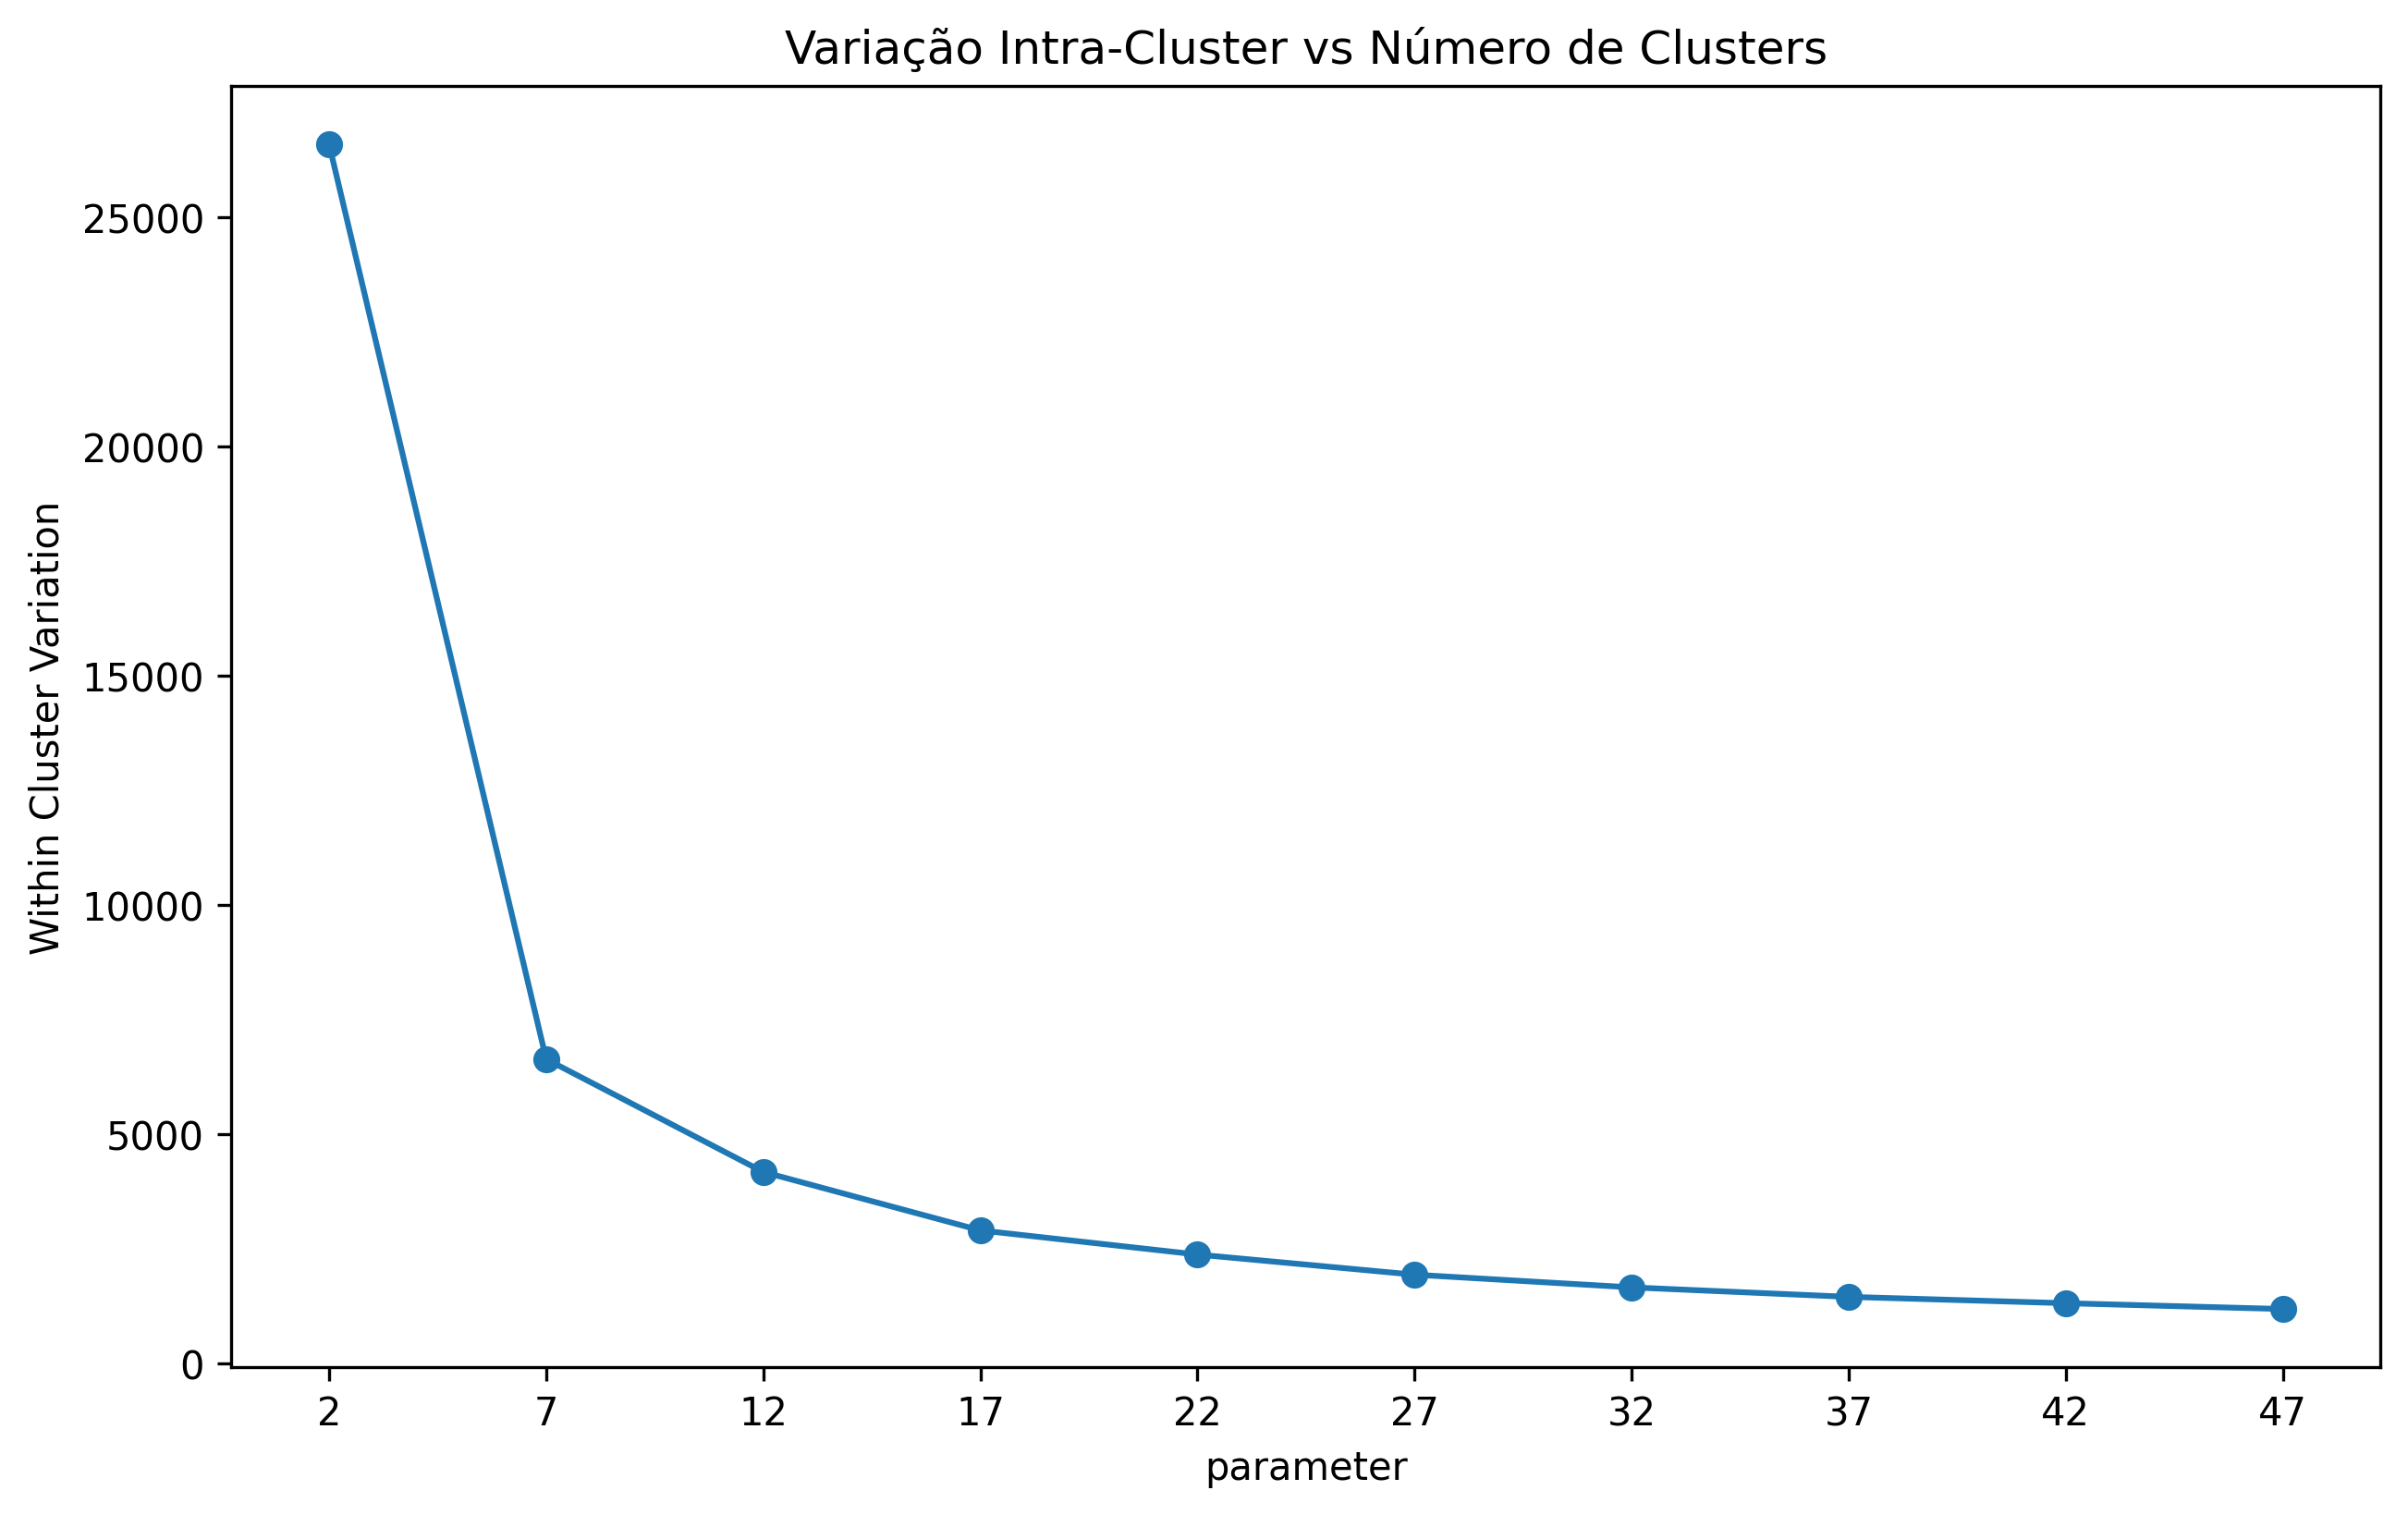
\includegraphics[width=0.8\textwidth]{../figures/5/within_cluster_variation.png}
    \caption{Variação intra-cluster vs número de clusters (método do cotovelo)}
    \label{fig:elbow_method}
\end{figure}

\textbf{Escolha do número de clusters:}

Considerando o gráfico, um valor de k apropriado para o problema seria 12. A partir deste ponto, a distância média entre os pontos de uma classe e o centro do cluster reduz menos com o aumento do número de centróides. Antes dele, essa distância era grande demais.

Em outras palavras, o trade-off entre compressão e reprodutibilidade teria um "joelho" neste ponto. Intuitivamente, usaríamos esse gráfico identificando o ponto onde a curva muda de comportamento (de decréscimo acentuado para decréscimo gradual).

\begin{figure}[H]
    \centering
    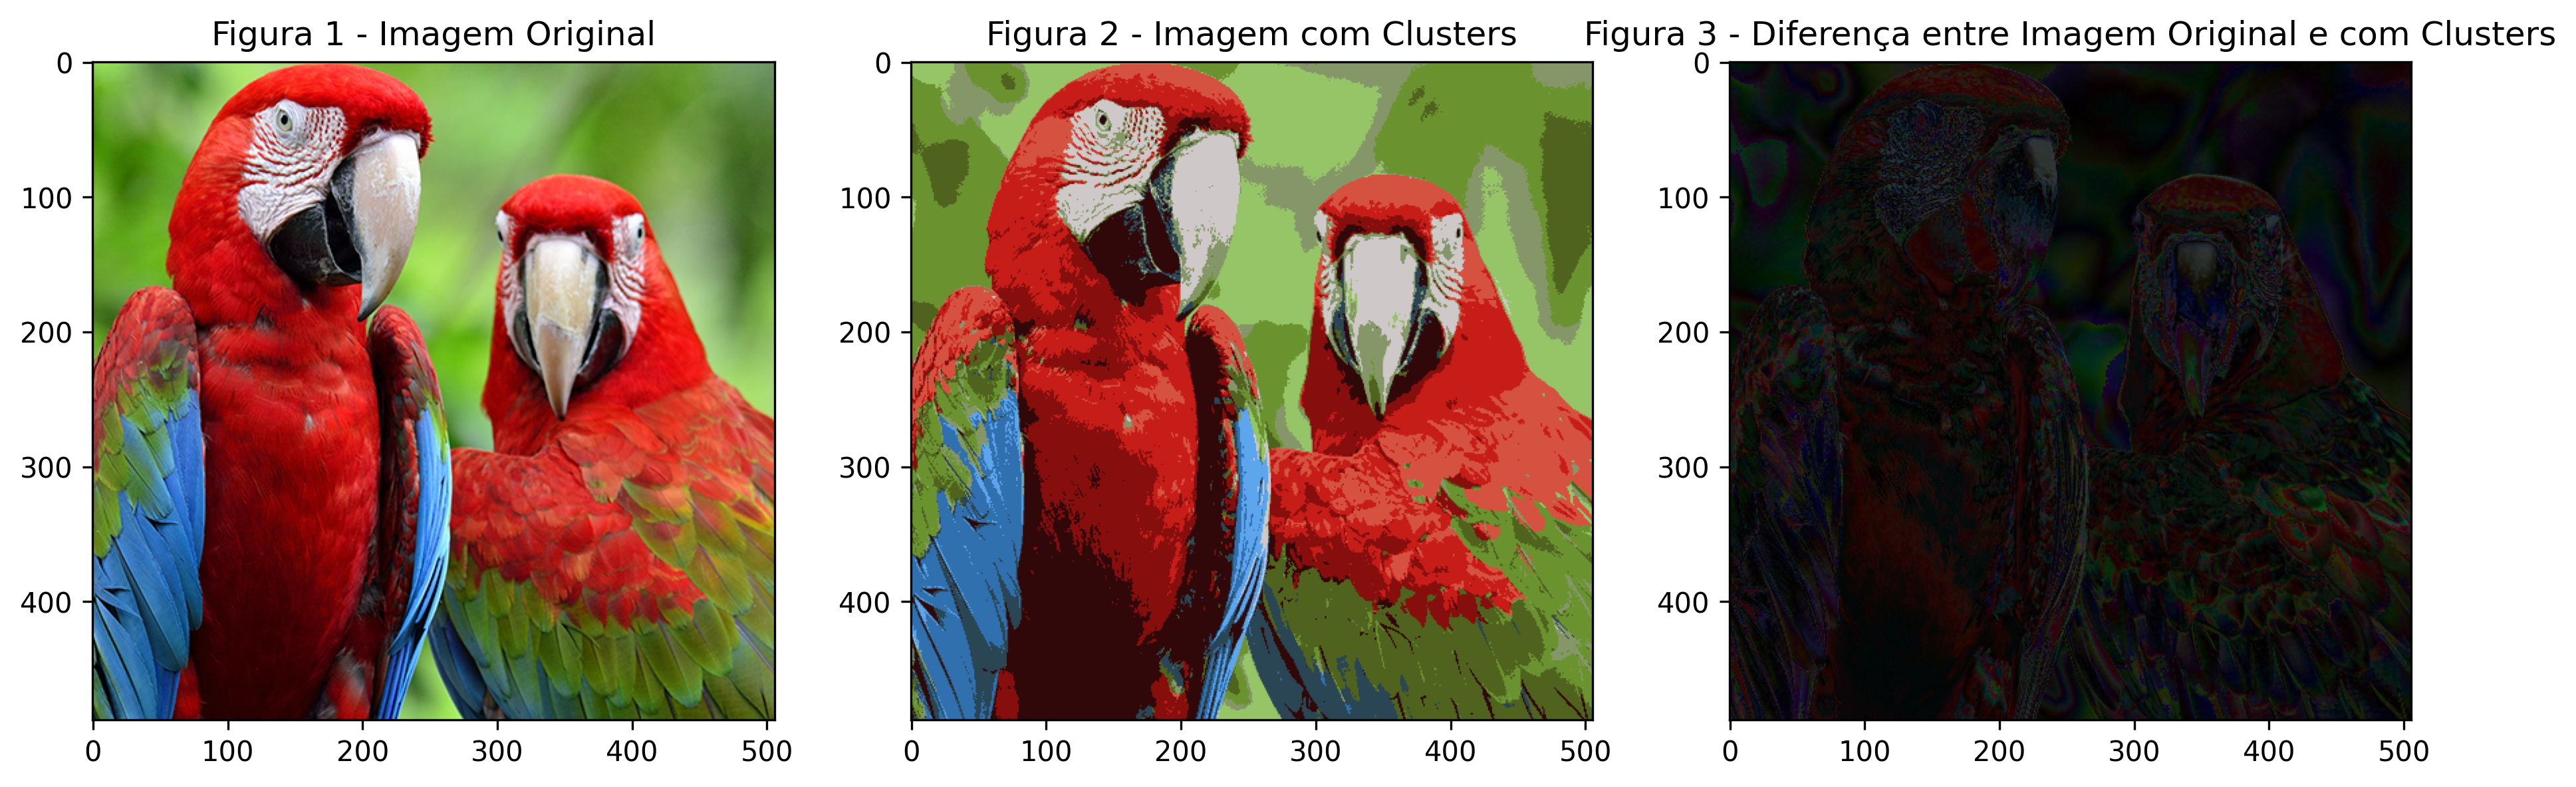
\includegraphics[width=0.9\textwidth]{../figures/5/optimal_k_result.png}
    \caption{Resultado com k=12 (valor otimizado)}
    \label{fig:optimal_k}
\end{figure}

A imagem acima apresenta o resultado da função \texttt{function\_1} para k=12, demonstrando que nesse ponto, a imagem mantém uma boa qualidade.